\section{Concept}
\label{sec:design}






TODO:
Rings
sysname
outer: environment
inner: system
interfaces between rings
mechanism








\paragraph{Mechanism}

We use the definition of \cite{} for Mechanisms: "A mechanism is a confined conceptual element of a networked system that is bound to a realization as cooperating functional units; the special case of an isolated realization (single-node) is permitted."

Examples of such mechanisms are manifold and span all protocol- and system-layers, as the following selection of possible mechanisms shows:

\begin{itemize}
 \item Complete protocols: TCP, UDP, RTP, overlays, etc.
 \item Fine-grained protocol mechanisms: congestion control, fragmentation, load balancing, replication, etc.
 \item Network concepts: infrastructure-based, ad-hoc, partially meshed, delay tolerant (DTN), etc.
 \item Network technologies: Ethernet, LTE, IEEE 802.11, Bluetooth, etc.
 \item Security mechanisms: encryption, integrity protection, authentication, etc.
 \item System components: positioning (via WLAN, GSM or GPS), sensors, etc.
\end{itemize}

\subsection{Concept}
\label{sec:design:concept}

Any communication between different parties relies on one or many \textit{communication interfaces}.
Such an interface can be anything from set of rules governing the actual communication, such as protocols defined on the different layers of the network-stack-model, to implicit assumptions over the inner workings of peers in a network.
While the network stack itself already offers plenty of possibilities to intervene and modify a node's behavior, via the use of a \textit{network shim}, extending this line of thought to include the entirety of a node's behavior allows for novel approaches to the problem of communication adjustments.

The advantage of such a holisitc approach to communication behavior can be seen in the fact, that it allows us to also alter behavior of network participant which are incapable or unwilling to modify their own operation.
This could be due to a network participant being built upon a proprietary frameworks, which disallows the modification of the device after sale, or simply due to the manufacturer dropping support.
In such a case we are unable to modify the node itself, but we may still be capable of modifying its environment to enforce the desired adaption in its behavior.

This change can be thought of as an ''outer'' level of the communication infrastructure enveloping an ''innter'' level and thus forcing a change.
When faced with a closed application, we might modify the operating system to force the applications behavior to change by, for example, modifying the network stack to transparently wrap connection in a VPN.

If the whole device is unmodifiable, but the network is under our control, then we may utilize the network  to force the device to behave in a certain way, e.g. by placing gateway-servers inside  the network who can transparently alter traffic flows.

If even the network is outside our control, then we may still affect change by modifying, or replacing the communication partner/backend with which the device is communicating.
By knowing the communication protocols and crafting messages in such a way that will trigger certain behavior in the device.

In addition to classic wireless technologies such as WLAN and LTE, multi-RATs are becoming the standard in mobile communication in the context of 5G. 
At the same time, these multi-RATs can so far only be used within the scope of the functionality implemented in the technology and do not allow fine-grained user control over the parameters of the lower layers.
It is desirable not only to combine the standard technologies advantageously, as can be done by multipath transport protocols, but also to adapt the individual RATs at runtime through targeted modification at the lower layers in such a way that the cooperation between the RATs is further optimised. 
For example, some RATs can no longer be used sensibly if, due to harsh environmental conditions, an excessively high packet error rate occurs even with robust coding and modulation procedures. A solution approach for this could be:
\begin{itemize}
\item the combination of several RATs with dynamic splitting of data between the RATs,
\item splitting data packets into smaller units to maximise their reliable transmission, and 
\item the use of customised error correction procedures across all RATs to ensure e.g. mission critical requirements.
\end{itemize}

In order to make the aforementioned adaptations also on legacy devices, it is necessary to migrate novel functionality to existing devices, for example by implanting an error correction mechanism that covers all RATs simultaneously, or configuring a RAT also outside the configuration predefined by the equipment provider. 

\paragraph{OS-side Adaption}

From the OS view the possible 

\paragraph{Network-side Adaption}

From the network point of view a legacy device can be handled as blackbox and arriving data can be interpreted as byte string which can be eg. split and send over different RATs. 
All additional concepts and improvements like custom error correction could also be applied on lower layer. 
This is the easiest way for a conceptional view of the data transmission and offers many possibilities of improvements.
But two possibilities exist:
1. The backend or target of the communication understands this change, then it can be easily done by the enveloping network
2. The backend or target of the communication is as legacy as the enveloped system, then the backend must also be encapsulated by an envelopment and the operations must be reversed.  

Alternatively, if the specific communication protocol used by the legacy device is known, the network can influence the device's operation by crafting packets which trigger changes in legacy device behaviour.

In a scenario, which includes both transition-enabled, and legacy devices, this enables the network-controller to orchestrate the legacy device's behaviour in such a way, the allows for smooth operation of such a heterogeneous network.
For example, the network could strategically drop packets, modify flow-control header fields or restrict bandwidth to ensure that a legacy device does not attempt to utilise more network bandwidth that would be appropriate.

Furthermore, when the device's internal behaviour depends directly on received packets, for example if the device receives commands via the network, then these packets can be crafted in such a way, that limit traffic generation on the device itself.
In section \ref{sec:implementation:treetalker}, we will go into a concrete example for the approach, which involves a distributed sensor-network connected by the low bandwidth LoRa wireless-communication standard.

%\subsection{Concept}
%\label{sec:design:concept}

%\paragraph{OS-side}

%Design graph for OS-side concept
%+ description of the concept from this point of view

%\paragraph{Network-side}

%Design graph for Network-side concept
%+ description of the concept from this point of view

%%\paragraph{Holistic Concept}

%Merging both concepts results in a general approach and in the concept of mechanism migration to legacy devices.


\begin{figure}
    \centering
    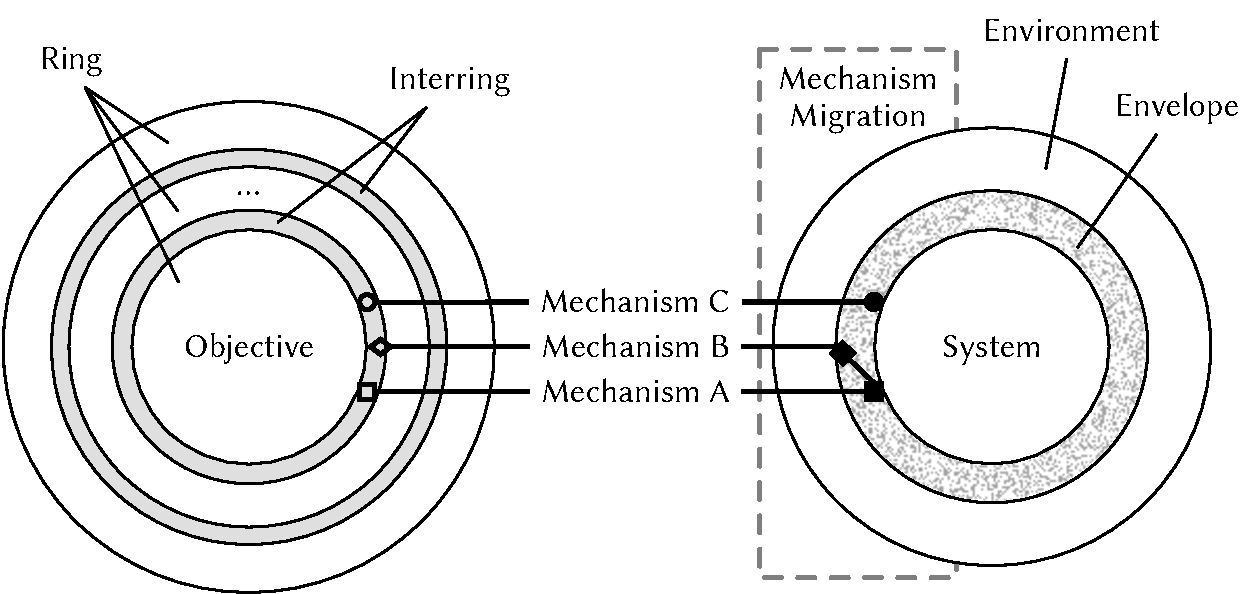
\includegraphics[width=.8\linewidth]{figures/MechanismMigration.pdf}
    \caption{Mechanism migration to a legacy device with transition-enabled environment}
    \label{fig:bigpicture}
\end{figure}

